\documentclass{article}
% Adjust the relative path to point to the latex-templates directory from:
% content/resources/study-materials/32-ict/sem-4/4343202-computer-networking/

% content/resources/templates/preamble.tex
\usepackage[margin=0.6in]{geometry}
\author{Milav Dabgar}
\usepackage{amsmath,amssymb,amsthm}
\usepackage{booktabs}
\usepackage{multirow}
\usepackage{xcolor}
\usepackage{tcolorbox}
\tcbuselibrary{breakable,skins}
\usepackage[colorlinks=true,linkcolor=blue]{hyperref}
\usepackage{titlesec}
\usepackage{enumitem}
\usepackage{tikz}
\usepackage{pgfplots}
\usepackage{circuitikz}
\usepackage[version=4]{mhchem}
\usepackage{longtable}
\usepackage{array}
\usepackage{float}
\usepackage{caption}
\usepackage{listings}

\lstset{
  basicstyle=\small\ttfamily,
  breaklines=true,
  breakatwhitespace=false,
  postbreak=\mbox{\textcolor{red}{$\hookrightarrow$}\space},
  float=false,
  numbers=left,
  numberstyle=\tiny\color{gray},
  numbersep=10pt,
  xleftmargin=2em,
  keywordstyle=\color{blue},
  commentstyle=\color{green!60!black},
  stringstyle=\color{purple},
  backgroundcolor=\color{gray!5},
  showstringspaces=false,
  tabsize=2,
  captionpos=b,
  keepspaces=true,
  columns=flexible
}

\pgfplotsset{compat=1.18}
\usetikzlibrary{shapes,arrows,positioning,calc,patterns,decorations.pathmorphing,decorations.markings,arrows.meta}

% Color scheme
\definecolor{headcolor}{RGB}{0,102,204}
\definecolor{keycolor}{RGB}{220,20,60}
\definecolor{solutioncolor}{RGB}{34,139,34}
\definecolor{mnemoniccolor}{RGB}{148,0,211}
\definecolor{codecolor}{RGB}{0,0,100}

% Spacing
\setlength{\parskip}{3pt}
\setlist[itemize]{nosep}
\setlist[enumerate]{nosep}

% Title formatting
\titleformat{\section}{\Large\bfseries\color{headcolor}}{\thesection}{1em}{}
\titleformat{\subsection}{\large\bfseries\color{headcolor}}{\thesubsection}{1em}{}

% Pandoc tightlist compatibility
\providecommand{\tightlist}{%
  \setlength{\itemsep}{0pt}\setlength{\parskip}{0pt}}

% Pandoc longtable compatibility
\newcounter{none}
\def\thenone{}


% content/resources/templates/english-boxes.tex

% Custom environments
\newtcolorbox{solutionbox}{
 breakable,
 enhanced,
 colback=solutioncolor!5!white,
 colframe=solutioncolor!75!black,
 fonttitle=\bfseries,
 title=Solution
}

\newtcolorbox{solutionboxnobreak}{
 colback=solutioncolor!5!white,
 colframe=solutioncolor!75!black,
 fonttitle=\bfseries,
 title=Solution
}

\newtcolorbox{keyformula}{
 breakable,
 enhanced,
 colback=keycolor!5!white,
 colframe=keycolor!75!black,
 fonttitle=\bfseries,
 title=Key Formula
}

\newtcolorbox{mnemonicboxenv}{
 breakable,
 enhanced,
 colback=mnemoniccolor!5!white,
 colframe=mnemoniccolor!75!black,
 fonttitle=\bfseries,
 title=Mnemonic
}

\newcommand{\mnemonicbox}[1]{%
  \begin{mnemonicboxenv}
    #1
  \end{mnemonicboxenv}
}


% Custom commands for GTU solutions
% This file defines semantic commands for consistent formatting

% Question command with automatic formatting
\newcommand{\question}[2]{%
  \section*{Question #1}%
  \textbf{#2}%
}

% OR question variant
\newcommand{\questionor}[2]{%
  \section*{Question #1 OR}%
  \textbf{#2}%
}

% Proper table environment with caption
\newenvironment{answertable}[1]{%
  \begin{table}[htbp]
  \centering
  \caption{#1}
}{%
  \end{table}
}

% Proper figure environment for diagrams
\newenvironment{answerdiagram}[1]{%
  \begin{figure}[htbp]
  \centering
  \caption{#1}
}{%
  \end{figure}
}

% Semantic markup for key terms
\newcommand{\keyword}[1]{\textbf{#1}}
\newcommand{\code}[1]{\texttt{#1}}
\newcommand{\classname}[1]{\texttt{#1}}
\newcommand{\methodname}[1]{\texttt{#1}}

% Proper quotation marks
\newcommand{\mnemonic}[1]{``#1''}


\title{Computer Networking (4343202) -- Summer 2024 Solution}
\date{June 13, 2024}

\begin{document}
\maketitle

\questionmarks{1(a)}{3}{Explain packet switching network.}

\begin{solutionbox}
Packet switching is a network communication method where data is divided into small packets before transmission.

\textbf{Packet Switching Process:}

\begin{center}
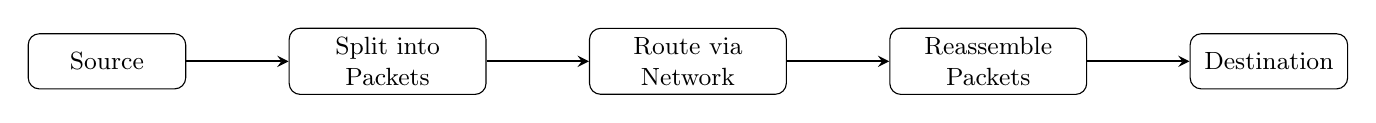
\begin{tikzpicture}[node distance=1.3cm, >=stealth, every node/.style={font=\small}]
    \node [draw, rectangle, rounded corners, minimum width=2cm, minimum height=0.7cm] (source) {Source};
    \node [draw, rectangle, rounded corners, minimum width=2.5cm, minimum height=0.7cm, right=of source, align=center] (split) {Split into\\Packets};
    \node [draw, rectangle, rounded corners, minimum width=2.5cm, minimum height=0.7cm, right=of split, align=center] (route) {Route via\\Network};
    \node [draw, rectangle, rounded corners, minimum width=2.5cm, minimum height=0.7cm, right=of route, align=center] (reassemble) {Reassemble\\Packets};
    \node [draw, rectangle, rounded corners, minimum width=2cm, minimum height=0.7cm, right=of reassemble] (dest) {Destination};
    
    \draw [->, thick] (source) -- (split);
    \draw [->, thick] (split) -- (route);
    \draw [->, thick] (route) -- (reassemble);
    \draw [->, thick] (reassemble) -- (dest);
\end{tikzpicture}
\captionof{figure}{Packet Switching Network}
\end{center}

\begin{itemize}
    \item \keyword{Independent routing}: Each packet travels independently through network
    \item \keyword{Flexible paths}: Packets can take different routes to reach destination
    \item \keyword{Efficiency}: Better utilization of network bandwidth
\end{itemize}
\end{solutionbox}

\begin{mnemonicbox}
\mnemonic{DIVE: Data Into Various Elements}
\end{mnemonicbox}

\questionmarks{1(b)}{4}{Write functional description of any four layers of OSI reference model.}

\begin{solutionbox}
The OSI model divides network communication into seven distinct layers, each with specific functions.

\begin{center}
\captionof{table}{OSI Layer Functions}
\begin{tabulary}{\linewidth}{|L|L|L|}
\hline
\textbf{Layer} & \textbf{Function} & \textbf{Key Protocols} \\ \hline
Application & Provides network services directly to user applications & HTTP, FTP, SMTP \\ \hline
Presentation & Translates, encrypts, and compresses data & SSL, TLS, JPEG \\ \hline
Session & Establishes, manages, and terminates connections & NetBIOS, RPC \\ \hline
Transport & Ensures reliable end-to-end data transfer & TCP, UDP \\ \hline
\end{tabulary}
\end{center}

\begin{itemize}
    \item \keyword{Application layer}: Interface between network and applications
    \item \keyword{Presentation layer}: Data formatting and encryption
    \item \keyword{Session layer}: Dialog control and synchronization
    \item \keyword{Transport layer}: End-to-end connection and reliability
\end{itemize}
\end{solutionbox}

\begin{mnemonicbox}
\mnemonic{All People Seem To Need Data Processing}
\end{mnemonicbox}

\questionmarks{1(c)}{7}{Explain Network topologies and with diagram.}

\begin{solutionbox}
Network topology refers to the physical or logical arrangement of devices in a network.

\begin{center}
\captionof{table}{Network Topology Comparison}
\begin{tabulary}{\linewidth}{|L|L|L|}
\hline
\textbf{Topology} & \textbf{Advantages} & \textbf{Disadvantages} \\ \hline
Bus & Simple, inexpensive & Single point of failure \\ \hline
Star & Easy troubleshooting, centralized & Hub/switch failure affects all \\ \hline
Ring & Equal access for all nodes & Single cable failure affects network \\ \hline
Mesh & High reliability, no traffic problems & Expensive, complex \\ \hline
Tree & Easily expandable, structured & Dependent on root, complex \\ \hline
\end{tabulary}
\end{center}

\textbf{Diagram:}

\begin{center}
\begin{tikzpicture}[node distance=2cm]
    % Bus Topology
    \node at (0,3.5) {\textbf{BUS TOPOLOGY}};
    \node [gtu block, minimum width=0.8cm, minimum height=0.6cm] (B1) at (-3,2) {N1};
    \node [gtu block, minimum width=0.8cm, minimum height=0.6cm] (B2) at (-1,2) {N2};
    \node [gtu block, minimum width=0.8cm, minimum height=0.6cm] (B3) at (1,2) {N3};
    \node [gtu block, minimum width=0.8cm, minimum height=0.6cm] (B4) at (3,2) {N4};
    % Draw the bus line
    \draw [very thick] (-3.5,1.5) -- (3.5,1.5);
    % Connect nodes to bus
    \draw [thick] (B1.south) -- (B1.south |- 0,1.5);
    \draw [thick] (B2.south) -- (B2.south |- 0,1.5);
    \draw [thick] (B3.south) -- (B3.south |- 0,1.5);
    \draw [thick] (B4.south) -- (B4.south |- 0,1.5);
    
    % Star Topology
    \node at (0,-0.5) {\textbf{STAR TOPOLOGY}};
    \node [gtu block] (Hub) at (0,-2) {Hub/Switch};
    \node [gtu block, minimum width=0.8cm] (S1) at (-2,-2) {N1};
    \node [gtu block, minimum width=0.8cm] (S2) at (0,-3.5) {N2};
    \node [gtu block, minimum width=0.8cm] (S3) at (2,-2) {N3};
    \path [gtu arrow] (Hub) -- (S1);
    \path [gtu arrow] (Hub) -- (S2);
    \path [gtu arrow] (Hub) -- (S3);
\end{tikzpicture}
\captionof{figure}{Network Topologies}
\end{center}

\begin{itemize}
    \item \keyword{Bus topology}: All devices connected to single cable
    \item \keyword{Star topology}: All devices connected to central hub/switch
    \item \keyword{Ring topology}: Devices connected in closed loop
    \item \keyword{Mesh topology}: Each device connected to every other device
    \item \keyword{Tree topology}: Hierarchical star networks connected via bus
\end{itemize}
\end{solutionbox}

\begin{mnemonicbox}
\mnemonic{BSRMT: Better Solutions Require Multiple Topologies}
\end{mnemonicbox}

\questionmarks{1(c OR)}{7}{Draw the diagram of TCP/IP protocol suite and explain the functions of Application Layer, Transport Layer and Network Layer in detail.}

\begin{solutionbox}
The TCP/IP protocol suite organizes network communication into four functional layers.

\textbf{Diagram:}

\begin{center}
\begin{tikzpicture}[node distance=0cm]
    \node [gtu block, minimum width=8cm, minimum height=1.2cm] (App) {APPLICATION LAYER};
    \node [below=0.1cm of App, font=\small] {(HTTP, FTP, SMTP, DNS, TELNET)};
    \node [gtu block, minimum width=8cm, minimum height=1.2cm, below=0.5cm of App] (Trans) {TRANSPORT LAYER};
    \node [below=0.1cm of Trans, font=\small] {(TCP, UDP)};
    \node [gtu block, minimum width=8cm, minimum height=1.2cm, below=0.5cm of Trans] (Net) {INTERNET LAYER};
    \node [below=0.1cm of Net, font=\small] {(IP, ICMP, ARP, RARP)};
    \node [gtu block, minimum width=8cm, minimum height=1.2cm, below=0.5cm of Net] (Link) {NETWORK ACCESS LAYER};
    \node [below=0.1cm of Link, font=\small] {(Ethernet, Wi-Fi, Token Ring)};
\end{tikzpicture}
\captionof{figure}{TCP/IP Protocol Suite}
\end{center}

\begin{center}
\captionof{table}{TCP/IP Layer Functions}
\begin{tabulary}{\linewidth}{|L|L|L|}
\hline
\textbf{Layer} & \textbf{Main Function} & \textbf{Key Protocols} \\ \hline
Application & Provides network services to applications & HTTP, FTP, SMTP \\ \hline
Transport & End-to-end communication, data flow control & TCP, UDP \\ \hline
Internet (Network) & Logical addressing and routing & IP, ICMP, ARP \\ \hline
\end{tabulary}
\end{center}

\begin{itemize}
    \item \keyword{Application Layer}: User interface to network, application-specific protocols
    \item \keyword{Transport Layer}: Reliable data transmission, error recovery, flow control
    \item \keyword{Network Layer}: Routing packets between networks, IP addressing
\end{itemize}
\end{solutionbox}

\begin{mnemonicbox}
\mnemonic{ATN works: Application, Transport, Network works together}
\end{mnemonicbox}

\questionmarks{2(a)}{3}{Compare connection-oriented protocol and connection less protocol.}

\begin{solutionbox}
Connection-oriented and connectionless protocols differ in how they handle data transmission.

\begin{center}
\captionof{table}{Connection-oriented vs Connectionless Protocols}
\begin{tabulary}{\linewidth}{|L|L|L|}
\hline
\textbf{Feature} & \textbf{Connection-oriented} & \textbf{Connectionless} \\ \hline
Connection & Establishes before transmission & No connection setup \\ \hline
Reliability & Guaranteed delivery & No delivery guarantee \\ \hline
Error checking & Extensive & Limited or none \\ \hline
Example & TCP & UDP \\ \hline
Usage & File transfer, web browsing & Streaming, DNS lookups \\ \hline
\end{tabulary}
\end{center}
\end{solutionbox}

\begin{mnemonicbox}
\mnemonic{REACH: Reliability Exists in All Connection Handshakes}
\end{mnemonicbox}

\questionmarks{2(b)}{4}{Explain Fast Ethernet \& Gigabit Ethernet.}

\begin{solutionbox}
Fast Ethernet and Gigabit Ethernet are higher-speed versions of the original Ethernet standard.

\begin{center}
\captionof{table}{Fast Ethernet vs Gigabit Ethernet}
\begin{tabulary}{\linewidth}{|L|L|L|}
\hline
\textbf{Feature} & \textbf{Fast Ethernet} & \textbf{Gigabit Ethernet} \\ \hline
Speed & 100 Mbps & 1000 Mbps (1 Gbps) \\ \hline
IEEE Standard & 802.3u & 802.3z/802.3ab \\ \hline
Cable Type & Cat5 UTP & Cat5e/Cat6 UTP, Fiber \\ \hline
Max Distance & 100m (copper) & 100m (copper), 5km (fiber) \\ \hline
\end{tabulary}
\end{center}

\begin{itemize}
    \item \keyword{Fast Ethernet}: 10x faster than original 10Base-T Ethernet
    \item \keyword{Gigabit Ethernet}: 10x faster than Fast Ethernet, backward compatible
    \item \keyword{Cabling}: Uses higher quality cabling to achieve greater speeds
    \item \keyword{Applications}: High-bandwidth network backbones, server connections
\end{itemize}
\end{solutionbox}

\begin{mnemonicbox}
\mnemonic{Fast Gets Going: 100 to 1000 Mbps progression}
\end{mnemonicbox}

\questionmarks{2(c)}{7}{Differentiate between Router, Hub and Switch.}

\begin{solutionbox}
Routers, hubs, and switches are network devices with different capabilities and functions.

\begin{center}
\captionof{table}{Router vs Hub vs Switch}
\begin{tabulary}{\linewidth}{|L|L|L|L|}
\hline
\textbf{Feature} & \textbf{Router} & \textbf{Hub} & \textbf{Switch} \\ \hline
OSI Layer & Network (3) & Physical (1) & Data Link (2) \\ \hline
Function & Connects networks & Connects devices & Connects devices \\ \hline
Data handling & Intelligent routing & Broadcasts to all & Sends to specific device \\ \hline
Security & Provides firewall & No security & Basic filtering \\ \hline
Addressing & Uses IP addresses & No addressing & Uses MAC addresses \\ \hline
Efficiency & High & Low & High \\ \hline
Intelligence & Smart & Dumb & Moderately smart \\ \hline
\end{tabulary}
\end{center}

\textbf{Diagram:}

\begin{center}
\begin{tikzpicture}[node distance=3cm]
    \node [gtu block, minimum width=2cm, minimum height=2cm, align=center] (R) {ROUTER\\[0.3cm]Routes\\between\\networks};
    \node [gtu block, minimum width=2cm, minimum height=2cm, align=center, right=of R] (H) {HUB\\[0.3cm]Shares\\signal\\to all\\ports};
    \node [gtu block, minimum width=2cm, minimum height=2cm, align=center, right=of H] (S) {SWITCH\\[0.3cm]Forwards\\to MAC\\address};
\end{tikzpicture}
\captionof{figure}{Network Devices Comparison}
\end{center}
\end{solutionbox}

\begin{mnemonicbox}
\mnemonic{RHS order: Router Has Smarts, Hub Shares Signal, Switch Sends Specifically}
\end{mnemonicbox}

\questionmarks{2(a OR)}{3}{Define E-mail system and list application of E-Mail.}

\begin{solutionbox}
An email system is a network service that allows exchange of digital messages between users.

\begin{center}
\captionof{table}{Email System Components}
\begin{tabulary}{\linewidth}{|L|L|}
\hline
\textbf{Component} & \textbf{Function} \\ \hline
Mail User Agent (MUA) & Email client software used by end-users \\ \hline
Mail Transfer Agent (MTA) & Server software that transfers emails \\ \hline
Mail Delivery Agent (MDA) & Delivers email to recipient's mailbox \\ \hline
Protocols & SMTP, POP3, IMAP \\ \hline
\end{tabulary}
\end{center}

\textbf{Applications of Email:}

\begin{itemize}
    \item Business communication
    \item Personal messaging
    \item File sharing
    \item Marketing and newsletters
    \item Notifications and alerts
\end{itemize}
\end{solutionbox}

\begin{mnemonicbox}
\mnemonic{BCPFN: Business Communication, Personal, Files, Newsletters}
\end{mnemonicbox}

\questionmarks{2(b OR)}{4}{Differentiate between IPv4 and IPv6.}

\begin{solutionbox}
IPv4 and IPv6 are Internet Protocol versions with significant differences.

\begin{center}
\captionof{table}{IPv4 vs IPv6}
\begin{tabulary}{\linewidth}{|L|L|L|}
\hline
\textbf{Feature} & \textbf{IPv4} & \textbf{IPv6} \\ \hline
Address length & 32-bit (4 bytes) & 128-bit (16 bytes) \\ \hline
Format & Dotted decimal (192.168.1.1) & Hexadecimal with colons (2001:0db8:85a3:0000:0000:8a2e:0370:7334) \\ \hline
Address space & \textasciitilde 4.3 billion addresses & 340 undecillion addresses \\ \hline
Security & Security added later & Built-in IPSec \\ \hline
Configuration & Manual or DHCP & Stateless auto-configuration \\ \hline
Header & Complex, variable & Simplified, fixed \\ \hline
\end{tabulary}
\end{center}

\begin{itemize}
    \item \keyword{IPv4}: Traditional addressing with limited space
    \item \keyword{IPv6}: Next-generation addressing with massive capacity
    \item \keyword{Transition}: Dual-stack, tunneling and translation mechanisms
\end{itemize}
\end{solutionbox}

\begin{mnemonicbox}
\mnemonic{4 SMALL, 6 HUGE: IPv4 Small address space, IPv6 Huge address space}
\end{mnemonicbox}

\questionmarks{2(c OR)}{7}{Discuss on Firewall with concept, principles, limitations, trusted system, Kerberos- concept in network security.}

\begin{solutionbox}
Firewalls are critical network security systems that monitor and control incoming and outgoing traffic.

\begin{center}
\captionof{table}{Firewall Types}
\begin{tabulary}{\linewidth}{|L|L|L|}
\hline
\textbf{Firewall Type} & \textbf{Function} & \textbf{Example} \\ \hline
Packet filtering & Examines packet headers & Router ACLs \\ \hline
Stateful inspection & Tracks connection state & Most hardware firewalls \\ \hline
Application layer & Inspects data contents & Web application firewalls \\ \hline
Next-generation & Combines multiple techniques & Palo Alto, Fortinet \\ \hline
\end{tabulary}
\end{center}

\textbf{Principles of Firewall:}

\begin{itemize}
    \item \keyword{Default deny}: Block everything unless explicitly allowed
    \item \keyword{Defense in depth}: Multiple security layers
    \item \keyword{Least privilege}: Minimal necessary access
\end{itemize}

\textbf{Limitations:}

\begin{itemize}
    \item Cannot protect against authorized users
    \item Limited against encrypted malicious traffic
    \item Performance impact on network
\end{itemize}

\textbf{Trusted Systems:}

\begin{itemize}
    \item Systems meeting specific security requirements
    \item Formal security policy enforcement
    \item Access control and authentication mechanisms
\end{itemize}

\textbf{Kerberos Concept:}

\begin{center}
\begin{tikzpicture}[node distance=3cm]
    \node [gtu block] (Client) {Client};
    \node [gtu block, right=of Client] (KDC) {KDC};
    \node [gtu block, right=of KDC] (Server) {Server};
    
    \path [gtu arrow, bend left=20] (Client) edge node[above] {Request} (KDC);
    \path [gtu arrow, bend left=20] (KDC) edge node[below] {Ticket} (Client);
    \path [gtu arrow, bend left=20] (Client) edge node[above] {Service Request} (Server);
    \path [gtu arrow, bend left=20] (Server) edge node[below] {Session Key} (Client);
\end{tikzpicture}
\captionof{figure}{Kerberos Authentication}
\end{center}

\begin{itemize}
    \item \keyword{Authentication protocol} using trusted third party
    \item \keyword{Ticket-based} access control system
    \item \keyword{Mutual authentication} between client and server
    \item \keyword{Time-sensitive} tickets prevent replay attacks
\end{itemize}
\end{solutionbox}

\begin{mnemonicbox}
\mnemonic{FLASK: Firewalls Lock Access, Secure with Kerberos}
\end{mnemonicbox}

\questionmarks{3(a)}{3}{Describe Sub-layers of Data link Layers.}

\begin{solutionbox}
The Data Link Layer in the OSI model is divided into two sublayers with distinct functions.

\begin{center}
\captionof{table}{Data Link Layer Sublayers}
\begin{tabulary}{\linewidth}{|L|L|L|}
\hline
\textbf{Sublayer} & \textbf{Function} & \textbf{Standards} \\ \hline
Logical Link Control (LLC) & Flow control, error checking & IEEE 802.2 \\ \hline
Media Access Control (MAC) & Channel access, addressing & IEEE 802.3, 802.11 \\ \hline
\end{tabulary}
\end{center}

\textbf{Diagram:}

\begin{center}
\begin{tikzpicture}[node distance=0cm]
    \node [gtu block, minimum width=8cm, minimum height=1cm] (Net) {NETWORK LAYER};
    \node [gtu block, minimum width=8cm, minimum height=1.5cm, below=0.1cm of Net, align=center] (LLC) {LOGICAL LINK CONTROL\\(LLC - 802.2)};
    \node [right=0.2cm of LLC, align=left, font=\small] {Flow control, Error handling\\Multiplexing, Connection mgmt};
    \node [gtu block, minimum width=8cm, minimum height=1.5cm, below=0.1cm of LLC, align=center] (MAC) {MEDIA ACCESS CONTROL\\(MAC - 802.3, 802.11)};
    \node [right=0.2cm of MAC, align=left, font=\small] {MAC addressing, Channel access\\Frame delimiting, Error detection};
    \node [gtu block, minimum width=8cm, minimum height=1cm, below=0.1cm of MAC] (Phy) {PHYSICAL LAYER};
\end{tikzpicture}
\captionof{figure}{Data Link Layer Sublayers}
\end{center}

\begin{itemize}
    \item \keyword{LLC}: Provides interface to network layer, error/flow control
    \item \keyword{MAC}: Handles physical addressing and media access
\end{itemize}
\end{solutionbox}

\begin{mnemonicbox}
\mnemonic{MAC LLCs order: MAC handles Lower Layer, LLC coordinates higher}
\end{mnemonicbox}

\questionmarks{3(b)}{4}{Explain IP layer protocols in detail.}

\begin{solutionbox}
The IP layer contains several key protocols that work together to facilitate internetwork communication.

\begin{center}
\captionof{table}{IP Layer Protocols}
\begin{tabulary}{\linewidth}{|L|L|L|}
\hline
\textbf{Protocol} & \textbf{Function} & \textbf{Key Features} \\ \hline
IP & Basic datagram delivery & Addressing, fragmentation, TTL \\ \hline
ICMP & Network diagnostics & Error reporting, ping, traceroute \\ \hline
ARP & Address resolution & Maps IP to MAC addresses \\ \hline
RARP & Reverse address resolution & Maps MAC to IP addresses \\ \hline
IGMP & Multicast group management & Manages host groups \\ \hline
\end{tabulary}
\end{center}

\begin{itemize}
    \item \keyword{IP}: Core protocol for addressing and routing packets
    \item \keyword{ICMP}: Error messages and operational information
    \item \keyword{ARP/RARP}: Address translation between layers
    \item \keyword{IGMP}: Manages multicast group memberships
\end{itemize}
\end{solutionbox}

\begin{mnemonicbox}
\mnemonic{I PAIR-up: IP, ICMP, ARP, RARP work as a team}
\end{mnemonicbox}

\questionmarks{3(c)}{7}{Describe different types of IP addressing schemes and explain various classes in classful IP addressing with example.}

\begin{solutionbox}
IP addressing schemes define how IP addresses are allocated and structured.

\begin{center}
\captionof{table}{IP Addressing Schemes}
\begin{tabulary}{\linewidth}{|L|L|L|}
\hline
\textbf{IP Addressing Scheme} & \textbf{Description} & \textbf{Example} \\ \hline
Classful & Traditional division into 5 classes & Class A: 10.0.0.0 \\ \hline
Classless (CIDR) & Flexible prefixes, more efficient & 192.168.1.0/24 \\ \hline
Private & Non-routable addresses for internal use & 192.168.0.0/16 \\ \hline
Special Purpose & Reserved for specific functions & 127.0.0.1 (localhost) \\ \hline
\end{tabulary}
\end{center}

\textbf{Classful IP Addressing:}

\begin{center}
\captionof{table}{Classful IP Address Classes}
\begin{tabulary}{\linewidth}{|L|L|L|L|L|L|L|}
\hline
\textbf{Class} & \textbf{First Bits} & \textbf{First Byte Range} & \textbf{Default Subnet Mask} & \textbf{Example} & \textbf{Networks} & \textbf{Hosts/Network} \\ \hline
A & 0 & 1-127 & 255.0.0.0 (/8) & 10.52.36.12 & 126 & 16,777,214 \\ \hline
B & 10 & 128-191 & 255.255.0.0 (/16) & 172.16.52.63 & 16,384 & 65,534 \\ \hline
C & 110 & 192-223 & 255.255.255.0 (/24) & 192.168.10.15 & 2,097,152 & 254 \\ \hline
D & 1110 & 224-239 & N/A (Multicast) & 224.0.0.5 & N/A & N/A \\ \hline
E & 1111 & 240-255 & N/A (Experimental) & 240.0.0.1 & N/A & N/A \\ \hline
\end{tabulary}
\end{center}

\begin{itemize}
    \item \keyword{Class A}: Large organizations, huge number of hosts
    \item \keyword{Class B}: Medium-sized organizations
    \item \keyword{Class C}: Small networks with few hosts
    \item \keyword{Class D}: Multicast groups
    \item \keyword{Class E}: Reserved for experimental use
\end{itemize}
\end{solutionbox}

\begin{mnemonicbox}
\mnemonic{All Businesses Care During Exams: Classes A, B, C, D, E}
\end{mnemonicbox}

\questionmarks{3(a OR)}{3}{Describe Digital Subscriber Line technology.}

\begin{solutionbox}
Digital Subscriber Line (DSL) is a technology that provides digital data transmission over telephone lines.

\begin{center}
\captionof{table}{DSL Types}
\begin{tabulary}{\linewidth}{|L|L|L|L|}
\hline
\textbf{DSL Type} & \textbf{Speed (Down/Up)} & \textbf{Distance} & \textbf{Application} \\ \hline
ADSL & 8 Mbps/1 Mbps & Up to 5.5 km & Home internet \\ \hline
SDSL & 2 Mbps/2 Mbps & Up to 3 km & Business \\ \hline
VDSL & 52 Mbps/16 Mbps & Up to 1.2 km & Video streaming \\ \hline
HDSL & 2 Mbps/2 Mbps & Up to 3.6 km & T1/E1 replacement \\ \hline
\end{tabulary}
\end{center}

\textbf{Diagram:}

\begin{center}
\begin{tikzpicture}[node distance=3cm]
    \node [gtu block] (Home) {HOME};
    \node [gtu block, right=2cm of Home] (Modem) {DSL MODEM};
    \node [gtu block, right=3cm of Modem] (DSLAM) {DSLAM};
    \node [gtu block, right=2cm of DSLAM] (ISP) {INTERNET};
    
    \path [gtu arrow] (Home) -- (Modem);
    \path [gtu arrow] (Modem) -- node[above] {Copper Line (POTS)} (DSLAM);
    \path [gtu arrow] (DSLAM) -- (ISP);
    \node [below=0.3cm of DSLAM] {ISP};
\end{tikzpicture}
\captionof{figure}{DSL System}
\end{center}

\begin{itemize}
    \item \keyword{Spectrum usage}: Uses higher frequencies than voice
    \item \keyword{Always-on}: Continuous connection, no dial-up
    \item \keyword{xDSL}: Family of technologies with different capabilities
\end{itemize}
\end{solutionbox}

\begin{mnemonicbox}
\mnemonic{SAVE Bandwidth: SDSL, ADSL, VDSL, HDSL Bandwidth options}
\end{mnemonicbox}

\questionmarks{3(b OR)}{4}{Discuss Cable Modem System.}

\begin{solutionbox}
Cable modem system provides internet access through the same coaxial cable used for cable TV.

\begin{center}
\captionof{table}{Cable Modem Components}
\begin{tabulary}{\linewidth}{|L|L|}
\hline
\textbf{Component} & \textbf{Function} \\ \hline
Cable modem & User-end device converting digital signals \\ \hline
CMTS & Cable Modem Termination System at provider end \\ \hline
HFC & Hybrid Fiber-Coaxial network infrastructure \\ \hline
DOCSIS & Data Over Cable Service Interface Specification \\ \hline
\end{tabulary}
\end{center}

\textbf{Diagram:}

\begin{center}
\begin{tikzpicture}[node distance=3cm]
    \node [gtu block] (Home) {HOME MODEM};
    \node [gtu block, right=2.5cm of Home] (Node) {NODE};
    \node [gtu block, right=3cm of Node] (CMTS) {ISP CMTS};
    \node [gtu block, right=2cm of CMTS] (Internet) {INTERNET};
    
    \path [gtu arrow] (Home) -- node[above] {COAX} (Node);
    \path [gtu arrow] (Node) -- node[above] {FIBER} (CMTS);
    \path [gtu arrow] (CMTS) -- (Internet);
    \node [below=0.3cm of Node] {NEIGHBORHOOD};
    \node [below=0.3cm of CMTS] {HEAD-END};
\end{tikzpicture}
\captionof{figure}{Cable Modem System}
\end{center}

\begin{itemize}
    \item \keyword{Shared medium}: Neighborhood shares bandwidth
    \item \keyword{Asymmetric}: Typically faster download than upload
    \item \keyword{DOCSIS standards}: Evolving specifications for speed/features
\end{itemize}
\end{solutionbox}

\begin{mnemonicbox}
\mnemonic{CHAMPS: Cable, HFC, Access, Modem, Provider, Shared}
\end{mnemonicbox}

\questionmarks{3(c OR)}{7}{Describe in brief all Transmission Media.}

\begin{solutionbox}
Transmission media are the physical paths through which data travels in a network.

\begin{center}
\captionof{table}{Transmission Media Types}
\begin{tabulary}{\linewidth}{|L|L|L|L|L|}
\hline
\textbf{Medium Type} & \textbf{Examples} & \textbf{Max Distance} & \textbf{Max Bandwidth} & \textbf{Application} \\ \hline
\multicolumn{5}{|c|}{\textbf{Guided (Wired)}} \\ \hline
Twisted Pair & UTP, STP & 100m & 10 Gbps & Office LANs \\ \hline
Coaxial Cable & RG-6, RG-59 & 500m & 10 Gbps & Cable TV, Internet \\ \hline
Fiber Optic & Single-mode, Multi-mode & 100km+ & 100+ Tbps & Backbones, Long-distance \\ \hline
\multicolumn{5}{|c|}{\textbf{Unguided (Wireless)}} \\ \hline
Radio Waves & WiFi, Cellular & 100m-50km & 600 Mbps & Wireless networks \\ \hline
Microwaves & Terrestrial, Satellite & Line of sight & 10 Gbps & Point-to-point links \\ \hline
Infrared & IrDA & 1m & 16 Mbps & Remote controls \\ \hline
\end{tabulary}
\end{center}

\begin{itemize}
    \item \keyword{Guided media}: Physical paths confining signals
    \item \keyword{Unguided media}: Wireless transmission through air/vacuum
    \item \keyword{Characteristics}: Bandwidth, attenuation, noise immunity, cost
\end{itemize}
\end{solutionbox}

\begin{mnemonicbox}
\mnemonic{TRIM-CWF: Twisted, Radio, Infrared, Microwave, Coaxial, Wireless, Fiber}
\end{mnemonicbox}

\questionmarks{4(a)}{3}{Write note on DNS.}

\begin{solutionbox}
Domain Name System (DNS) translates human-friendly domain names to IP addresses.

\begin{center}
\captionof{table}{DNS Components}
\begin{tabulary}{\linewidth}{|L|L|}
\hline
\textbf{Component} & \textbf{Function} \\ \hline
Domain Name & Hierarchical, readable address (www.example.com) \\ \hline
DNS Server & Resolves domain names to IP addresses \\ \hline
Root Server & Top of DNS hierarchy, points to TLDs \\ \hline
TLD Server & Manages top-level domains (.com, .org) \\ \hline
Record Types & A, AAAA, MX, CNAME, NS, PTR, etc. \\ \hline
\end{tabulary}
\end{center}

\textbf{Diagram:}

\begin{center}
\begin{tikzpicture}[node distance=2.5cm]
    \node [gtu block] (Client) {CLIENT};
    \node [gtu block, right=of Client] (Local) {LOCAL DNS};
    \node [gtu block, above right=1cm and 1.5cm of Local] (Root) {ROOT DNS};
    \node [gtu block, below right=1cm and 1.5cm of Local] (TLD) {TLD};
    \node [gtu block, right=of TLD] (Domain) {DOMAIN SERVER};
    
    \path [gtu arrow, bend left=15] (Client) edge node[above] {1. Query} (Local);
    \path [gtu arrow, bend left=15] (Local) edge node[below] {8. Response} (Client);
    \path [gtu arrow, bend left=15] (Local) edge node[above left] {2} (Root);
    \path [gtu arrow, bend left=15] (Root) edge node[below right] {3} (Local);
    \path [gtu arrow, bend left=15] (Local) edge node[above left] {4} (TLD);
    \path [gtu arrow, bend left=15] (TLD) edge node[below right] {5} (Local);
    \path [gtu arrow, bend left=15] (Local) edge node[above] {6} (Domain);
    \path [gtu arrow, bend left=15] (Domain) edge node[below] {7} (Local);
\end{tikzpicture}
\captionof{figure}{DNS Resolution Process}
\end{center}

\begin{itemize}
    \item \keyword{Distributed database}: Hierarchical, globally distributed
    \item \keyword{Caching}: Improves performance, reduces load
    \item \keyword{Critical infrastructure}: Essential for Internet functionality
\end{itemize}
\end{solutionbox}

\begin{mnemonicbox}
\mnemonic{DIRT: Domain names Into Routable TCP/IP}
\end{mnemonicbox}

\questionmarks{4(b)}{4}{Explain File Transfer Protocol.}

\begin{solutionbox}
File Transfer Protocol (FTP) enables transfer of files between client and server over a network.

\begin{center}
\captionof{table}{FTP Features}
\begin{tabulary}{\linewidth}{|L|L|}
\hline
\textbf{Feature} & \textbf{Description} \\ \hline
Port & Control: 21, Data: 20 \\ \hline
Mode & Active and Passive \\ \hline
Security & Basic (clear text), or FTPS/SFTP for encryption \\ \hline
Commands & GET, PUT, LIST, DELETE, etc. \\ \hline
Connection & Uses separate control and data connections \\ \hline
\end{tabulary}
\end{center}

\textbf{Diagram:}

\begin{center}
\begin{tikzpicture}[node distance=4cm]
    \node [gtu block] (Client) {CLIENT};
    \node [gtu block, right=of Client] (Server) {SERVER};
    
    \path [gtu arrow, bend left=20] (Client) edge node[above] {Control (Port 21)} (Server);
    \path [gtu arrow, bend left=20] (Server) edge node[below] {Data (Port 20)} (Client);
\end{tikzpicture}
\captionof{figure}{FTP Dual Connection}
\end{center}

\begin{itemize}
    \item \keyword{Dual channel}: Control channel and data channel
    \item \keyword{Authentication}: Username/password required
    \item \keyword{Modes}: ASCII (text) or Binary (raw data)
    \item \keyword{Active vs Passive}: Different connection establishment methods
\end{itemize}
\end{solutionbox}

\begin{mnemonicbox}
\mnemonic{CAPS: Control And Port Separation}
\end{mnemonicbox}

\questionmarks{4(c)}{7}{Classify different Internet Services and explain in detail.}

\begin{solutionbox}
Internet services provide various functionality over the network.

\begin{center}
\captionof{table}{Internet Service Categories}
\begin{tabulary}{\linewidth}{|L|L|L|L|}
\hline
\textbf{Service Category} & \textbf{Common Protocols} & \textbf{Description} & \textbf{Example Applications} \\ \hline
Communication & SMTP, POP3, IMAP & Exchange of messages & Email, Instant Messaging \\ \hline
Information Access & HTTP, HTTPS & Access to information resources & World Wide Web, Portals \\ \hline
File Sharing & FTP, BitTorrent, SMB & Transfer and sharing of files & File hosting, P2P sharing \\ \hline
Remote Access & SSH, Telnet, RDP & Access remote computers & Remote administration \\ \hline
Real-time Services & VoIP, WebRTC & Live communication & Video conferencing, VoIP \\ \hline
Domain Services & DNS, DHCP & Network infrastructure & Address resolution \\ \hline
\end{tabulary}
\end{center}

\textbf{Information Access Services (Web):}

\begin{itemize}
    \item \keyword{HTTP/HTTPS}: HyperText Transfer Protocol, foundation of web
    \item \keyword{HTML}: Document format for displaying content
    \item \keyword{Web browsers}: Client software to access and render web content
    \item \keyword{Web servers}: Hosts websites and applications
\end{itemize}

\textbf{Communication Services (Email):}

\begin{itemize}
    \item \keyword{SMTP}: For sending email
    \item \keyword{POP3/IMAP}: For receiving email
    \item \keyword{Components}: Mail user agents, transfer agents, delivery agents
\end{itemize}

\textbf{File Sharing Services:}

\begin{itemize}
    \item \keyword{FTP}: Traditional file transfer protocol
    \item \keyword{P2P}: Distributed file sharing without central server
    \item \keyword{Cloud storage}: Remote file storage and synchronization
\end{itemize}
\end{solutionbox}

\begin{mnemonicbox}
\mnemonic{CIFRRD: Communication, Information, File, Remote, Real-time, Domain}
\end{mnemonicbox}

\questionmarks{4(a OR)}{3}{Explain Mail Protocols.}

\begin{solutionbox}
Mail protocols facilitate electronic messaging between users.

\begin{center}
\captionof{table}{Mail Protocols}
\begin{tabulary}{\linewidth}{|L|L|L|L|}
\hline
\textbf{Protocol} & \textbf{Function} & \textbf{Port} & \textbf{Direction} \\ \hline
SMTP & Simple Mail Transfer Protocol & 25, 587 & Sending mail \\ \hline
POP3 & Post Office Protocol v3 & 110 & Retrieving mail \\ \hline
IMAP & Internet Message Access Protocol & 143 & Advanced mail retrieval \\ \hline
MIME & Multipurpose Internet Mail Extensions & N/A & Encoding attachments \\ \hline
\end{tabulary}
\end{center}

\textbf{Diagram:}

\begin{center}
\begin{tikzpicture}[node distance=4cm]
    \node [gtu block] (Sender) {Sender Client};
    \node [gtu block, right=of Sender] (Mail) {Mail Server};
    \node [gtu block, right=of Mail] (Receiver) {Receiver Client};
    
    \path [gtu arrow] (Sender) -- node[above] {SMTP} (Mail);
    \path [gtu arrow] (Mail) -- node[above] {POP3/IMAP} (Receiver);
\end{tikzpicture}
\captionof{figure}{Mail Protocol Flow}
\end{center}

\begin{itemize}
    \item \keyword{SMTP}: Outgoing mail delivery, push protocol
    \item \keyword{POP3}: Simple mail retrieval, downloads and deletes
    \item \keyword{IMAP}: Advanced retrieval, server-side storage, folders
    \item \keyword{MIME}: Extends email capability for non-text content
\end{itemize}
\end{solutionbox}

\begin{mnemonicbox}
\mnemonic{SIM-P: SMTP sends, IMAP manages, POP3 pulls}
\end{mnemonicbox}

\questionmarks{4(b OR)}{4}{Describe VOIP in brief.}

\begin{solutionbox}
Voice over Internet Protocol (VoIP) transmits voice communications over IP networks.

\begin{center}
\captionof{table}{VoIP Components}
\begin{tabulary}{\linewidth}{|L|L|}
\hline
\textbf{Component} & \textbf{Function} \\ \hline
Codec & Encodes/decodes voice signals \\ \hline
Signaling Protocol & Call setup/tear down (SIP, H.323) \\ \hline
Transport Protocol & Voice packet delivery (RTP) \\ \hline
QoS mechanism & Ensures voice quality \\ \hline
\end{tabulary}
\end{center}

\textbf{Diagram:}

\begin{center}
\begin{tikzpicture}[node distance=5cm]
    \node [gtu block, align=center] (Caller) {CALLER\\ENDPOINT};
    \node [gtu block, align=center, right=of Caller] (Callee) {CALLEE\\ENDPOINT};
    
    \path [gtu arrow, bend left=20] (Caller) edge node[above] {Internet/IP Network} (Callee);
    \path [gtu arrow, bend left=20] (Callee) edge node[below] {RTP Packets} (Caller);
\end{tikzpicture}
\captionof{figure}{VoIP Communication}
\end{center}

\begin{itemize}
    \item \keyword{Packetization}: Converts analog voice to digital packets
    \item \keyword{Benefits}: Cost savings, flexibility, integration with apps
    \item \keyword{Challenges}: Quality of service, latency, jitter, packet loss
\end{itemize}
\end{solutionbox}

\begin{mnemonicbox}
\mnemonic{PALS: Packets Allowing Live Speech}
\end{mnemonicbox}

\questionmarks{4(c OR)}{7}{Describe TCP and UDP protocols.}

\begin{solutionbox}
TCP and UDP are the primary transport layer protocols in the TCP/IP suite.

\begin{center}
\captionof{table}{TCP vs UDP}
\begin{tabulary}{\linewidth}{|L|L|L|}
\hline
\textbf{Feature} & \textbf{TCP} & \textbf{UDP} \\ \hline
Connection & Connection-oriented & Connectionless \\ \hline
Reliability & Guaranteed delivery & Best-effort delivery \\ \hline
Header size & 20-60 bytes & 8 bytes \\ \hline
Speed & Slower due to overhead & Faster with minimal overhead \\ \hline
Order & Maintains sequence & No sequence preservation \\ \hline
Flow control & Yes & No \\ \hline
Error recovery & Retransmission & None \\ \hline
Usage & Web, email, file transfer & Streaming, DNS, VoIP \\ \hline
\end{tabulary}
\end{center}

\textbf{TCP Three-Way Handshake:}

\begin{center}
\begin{tikzpicture}[node distance=5cm]
    \node [gtu block] (Client) {CLIENT};
    \node [gtu block, right=of Client] (Server) {SERVER};
    
    \path [gtu arrow] (Client) -- node[above, pos=0.3] {SYN} (Server);
    \path [gtu arrow] (Server) -- node[below, pos=0.7] {SYN-ACK} (Client);
    \path [gtu arrow] (Client) -- node[above, pos=0.5] {ACK} (Server);
\end{tikzpicture}
\captionof{figure}{TCP Three-Way Handshake}
\end{center}

\textbf{TCP Features:}

\begin{itemize}
    \item \keyword{Reliability}: Acknowledgments, retransmission
    \item \keyword{Flow control}: Window-based, prevents overwhelming
    \item \keyword{Congestion control}: Slow start, congestion avoidance
    \item \keyword{Connection management}: Establishment, maintenance, termination
\end{itemize}

\textbf{UDP Features:}

\begin{itemize}
    \item \keyword{Lightweight}: Minimal headers, no connection state
    \item \keyword{Low latency}: No handshaking or acknowledgments
    \item \keyword{No guarantees}: Data may arrive out of order, duplicated, or not at all
    \item \keyword{Broadcast/multicast}: Supports one-to-many transmission
\end{itemize}
\end{solutionbox}

\begin{mnemonicbox}
\mnemonic{CRUFS: Connection, Reliability, UDP Fast, Simple}
\end{mnemonicbox}

\questionmarks{5(a)}{3}{Describe Cryptography.}

\begin{solutionbox}
Cryptography is the science of secure communication techniques that protect information.

\begin{center}
\captionof{table}{Cryptography Types}
\begin{tabulary}{\linewidth}{|L|L|L|}
\hline
\textbf{Type} & \textbf{Description} & \textbf{Example} \\ \hline
Symmetric & Same key for encryption and decryption & AES, DES \\ \hline
Asymmetric & Different keys for encryption and decryption & RSA, ECC \\ \hline
Hash Functions & One-way functions, fixed output size & SHA-256, MD5 \\ \hline
Digital Signatures & Authentication and integrity verification & RSA signatures \\ \hline
\end{tabulary}
\end{center}

\begin{itemize}
    \item \keyword{Confidentiality}: Protect information from unauthorized access
    \item \keyword{Integrity}: Ensure information hasn't been altered
    \item \keyword{Authentication}: Verify identity of communicating parties
\end{itemize}
\end{solutionbox}

\begin{mnemonicbox}
\mnemonic{SHAPE: Symmetric, Hashing, Asymmetric, Protect, Encrypt}
\end{mnemonicbox}

\questionmarks{5(b)}{4}{Explain Social issues and Hacking also discuss its precautions.}

\begin{solutionbox}
Social issues in cybersecurity involve human manipulation and societal impacts of cyber threats.

\begin{center}
\captionof{table}{Social Issues in Cybersecurity}
\begin{tabulary}{\linewidth}{|L|L|L|}
\hline
\textbf{Social Issue} & \textbf{Description} & \textbf{Example} \\ \hline
Social Engineering & Manipulating people to reveal information & Phishing, pretexting \\ \hline
Privacy Concerns & Unauthorized data collection and use & Data breaches, surveillance \\ \hline
Digital Divide & Inequality in technology access & Limited Internet in rural areas \\ \hline
Cyberbullying & Using technology to harass others & Online harassment, threats \\ \hline
\end{tabulary}
\end{center}

\textbf{Hacking Types:}

\begin{itemize}
    \item \keyword{White Hat}: Ethical hacking, security improvement
    \item \keyword{Black Hat}: Malicious hacking, illegal activities
    \item \keyword{Grey Hat}: Mix of ethical and questionable actions
\end{itemize}

\textbf{Precautions:}

\begin{itemize}
    \item \keyword{Education}: Regular security awareness training
    \item \keyword{Strong Policies}: Clear security procedures and policies
    \item \keyword{Technical Controls}: Firewalls, antivirus, encryption
    \item \keyword{Regular Updates}: Patching systems against vulnerabilities
    \item \keyword{Monitoring}: Activity logs, intrusion detection
\end{itemize}
\end{solutionbox}

\begin{mnemonicbox}
\mnemonic{STEPS: Social engineering, Training, Encryption, Patches, Strong passwords}
\end{mnemonicbox}

\questionmarks{5(c)}{7}{Explain IP Security in detail.}

\begin{solutionbox}
IP Security (IPsec) is a protocol suite that secures communications at the IP layer.

\begin{center}
\captionof{table}{IPsec Components}
\begin{tabulary}{\linewidth}{|L|L|L|}
\hline
\textbf{Component} & \textbf{Function} & \textbf{Description} \\ \hline
AH & Authentication Header & Provides integrity and authentication \\ \hline
ESP & Encapsulating Security Payload & Provides confidentiality, integrity, authentication \\ \hline
IKE & Internet Key Exchange & Establishes and manages security associations \\ \hline
SA & Security Association & Security parameters for a connection \\ \hline
\end{tabulary}
\end{center}

\textbf{IPsec Modes:}

\begin{center}
\captionof{table}{IPsec Modes}
\begin{tabulary}{\linewidth}{|L|L|L|}
\hline
\textbf{Mode} & \textbf{Description} & \textbf{Application} \\ \hline
Transport & Protects payload only & Host-to-host communications \\ \hline
Tunnel & Protects entire packet & Gateway-to-gateway (VPN) \\ \hline
\end{tabulary}
\end{center}

\textbf{IPsec Services:}

\begin{itemize}
    \item \keyword{Authentication}: Verifies sender identity
    \item \keyword{Confidentiality}: Encrypts data to prevent eavesdropping
    \item \keyword{Integrity}: Ensures data hasn't been modified
    \item \keyword{Anti-replay}: Prevents packet replay attacks
\end{itemize}

\textbf{IPsec Implementation:}

\begin{itemize}
    \item \keyword{VPNs}: Secure remote access and site-to-site connections
    \item \keyword{L2TP/IPsec}: Combines tunneling with security
    \item \keyword{Authentication methods}: Pre-shared keys, certificates, Kerberos
\end{itemize}
\end{solutionbox}

\begin{mnemonicbox}
\mnemonic{ACCEPT: Authentication, Confidentiality, Cryptography, Encapsulation, Protocols, Tunnel}
\end{mnemonicbox}

\questionmarks{5(a OR)}{3}{Define Network Security and explain its elements.}

\begin{solutionbox}
Network security is the protection of network infrastructure, data, and access against unauthorized use, malfunction, modification, or destruction.

\begin{center}
\captionof{table}{Network Security Elements}
\begin{tabulary}{\linewidth}{|L|L|L|}
\hline
\textbf{Element} & \textbf{Description} & \textbf{Examples} \\ \hline
Access Control & Limiting network access & Passwords, multi-factor auth \\ \hline
Threat Prevention & Blocking attacks & Firewalls, IDS/IPS \\ \hline
Encryption & Securing data in transit & SSL/TLS, IPsec \\ \hline
Vulnerability Management & Identifying weaknesses & Scanning, patching \\ \hline
Monitoring & Observing network activity & SIEM, log analysis \\ \hline
\end{tabulary}
\end{center}

\begin{itemize}
    \item \keyword{Confidentiality}: Protecting information from unauthorized access
    \item \keyword{Integrity}: Ensuring information accuracy and reliability
    \item \keyword{Availability}: Maintaining systems accessible when needed
\end{itemize}
\end{solutionbox}

\begin{mnemonicbox}
\mnemonic{CIMA TV: Confidentiality, Integrity, Monitoring, Access control, Threats, Vulnerabilities}
\end{mnemonicbox}

\questionmarks{5(b OR)}{4}{Briefly describe the Information Technology (Amendment) Act, 2008, and its impact on cyber laws in India.}

\begin{solutionbox}
The IT (Amendment) Act, 2008 updated India's cyber laws to address emerging cybersecurity challenges.

\begin{center}
\captionof{table}{IT Amendment Act 2008 Key Aspects}
\begin{tabulary}{\linewidth}{|L|L|}
\hline
\textbf{Key Aspect} & \textbf{Description} \\ \hline
Cyber Crimes & Added new offenses, strengthened penalties \\ \hline
Electronic Evidence & Recognized digital evidence in court \\ \hline
Data Protection & Imposed obligations for sensitive data \\ \hline
Intermediary Liability & Defined responsibilities for service providers \\ \hline
\end{tabulary}
\end{center}

\textbf{Key Sections:}

\begin{itemize}
    \item \keyword{Section 43}: Penalties for unauthorized access, data theft
    \item \keyword{Section 66}: Computer-related offenses and punishments
    \item \keyword{Section 69}: Powers for interception and monitoring
    \item \keyword{Section 72A}: Protection of personal data privacy
\end{itemize}

\textbf{Impact on Cyber Laws:}

\begin{itemize}
    \item \keyword{Stronger enforcement}: Enhanced penalties for cyber crimes
    \item \keyword{Expanded scope}: Covered new technological developments
    \item \keyword{Corporate responsibility}: Required security practices for data
    \item \keyword{Global alignment}: Harmonized with international standards
\end{itemize}
\end{solutionbox}

\begin{mnemonicbox}
\mnemonic{SPEC: Security, Privacy, Evidence, Cyber crimes}
\end{mnemonicbox}

\questionmarks{5(c OR)}{7}{Explain Email security in terms of SMTP, PEM, PGP, S/MINE, spam.}

\begin{solutionbox}
Email security protects email content and accounts from unauthorized access and attacks.

\begin{center}
\captionof{table}{Email Security Technologies}
\begin{tabulary}{\linewidth}{|L|L|L|}
\hline
\textbf{Technology} & \textbf{Function} & \textbf{Features} \\ \hline
SMTP & Simple Mail Transfer Protocol & Basic email transmission, limited security \\ \hline
PEM & Privacy Enhanced Mail & Early email encryption standard \\ \hline
PGP & Pretty Good Privacy & End-to-end encryption, digital signatures \\ \hline
S/MIME & Secure/Multipurpose Internet Mail Extensions & Certificate-based encryption and signing \\ \hline
Anti-spam & Unwanted email filtering & Content filtering, blacklists, authentication \\ \hline
\end{tabulary}
\end{center}

\textbf{SMTP Security Issues:}

\begin{itemize}
    \item Originally designed without security
    \item Authentication extensions (AUTH) added later
    \item Vulnerable to eavesdropping without encryption
    \item Supports STARTTLS for encrypted transmission
\end{itemize}

\textbf{PGP Email Security:}

\begin{center}
\begin{tikzpicture}[node distance=5cm]
    \node [gtu block] (Sender) {SENDER};
    \node [gtu block, right=of Sender] (Receiver) {RECEIVER};
    
    \path [gtu arrow, bend left=20] (Sender) edge node[above, align=center] {Encrypted Email\\(Sign + Encrypt)} (Receiver);
    \path [gtu arrow, bend left=20] (Receiver) edge node[below, align=center] {Decrypt + Verify} (Sender);
\end{tikzpicture}
\captionof{figure}{PGP Email Security}
\end{center}

\textbf{S/MIME Features:}

\begin{itemize}
    \item Uses X.509 certificates for authentication
    \item Provides encryption and digital signatures
    \item Integrated into many email clients
    \item Requires certificate infrastructure
\end{itemize}

\textbf{Spam Protection:}

\begin{itemize}
    \item \keyword{Content filtering}: Analyzing message content
    \item \keyword{Sender verification}: SPF, DKIM, DMARC
    \item \keyword{Behavioral analysis}: Pattern recognition
    \item \keyword{Blacklists/whitelists}: Blocking/allowing specific senders
\end{itemize}

\textbf{Email Security Best Practices:}

\begin{itemize}
    \item \keyword{Encryption}: Ensure privacy of message content
    \item \keyword{Authentication}: Verify sender identity
    \item \keyword{Access controls}: Protect email accounts
    \item \keyword{Filtering}: Block malicious and unwanted messages
    \item \keyword{User education}: Recognize phishing attempts
\end{itemize}
\end{solutionbox}

\begin{mnemonicbox}
\mnemonic{SPEED: S/MIME, PGP, Encryption, Email security, DMARC}
\end{mnemonicbox}

\end{document}

